%%%%%%%%%%%%%%%%%%%%%%%%%%%%%%%%%%%%%%%%%%%%%%%%%%%%%%%%%%%%%%%%%%%%%%%%%%%%%%%%
%2345678901234567890123456789012345678901234567890123456789012345678901234567890
%        1         2         3         4         5         6         7         8

\documentclass[letterpaper, 10 pt, conference]{ieeeconf}  % Comment this line out
                                                          % if you need a4paper
%\documentclass[a4paper, 10pt, conference]{ieeeconf}      % Use this line for a4
                                                          % paper

\IEEEoverridecommandlockouts                              % This command is only
                                                          % needed if you want to
                                                          % use the \thanks command
\overrideIEEEmargins
% See the \addtolength command later in the file to balance the column lengths
% on the last page of the document

\usepackage[utf8]{inputenc}
\usepackage[T1]{fontenc}
\usepackage[english]{babel}
\usepackage{graphicx}
\usepackage{placeins}
\usepackage{amsmath}
\usepackage[table,xcdraw]{xcolor}
% The following packages can be found on http:\\www.ctan.org
% \usepackage{graphics} % for pdf, bitmapped graphics files
%\usepackage{epsfig} % for postscript graphics files
%\usepackage{mathptmx} % assumes new font selection scheme installed
%\usepackage{mathptmx} % assumes new font selection scheme installed
%\usepackage{amsmath} % assumes amsmath package installed
%\usepackage{amssymb}  % assumes amsmath package installed

\title{\LARGE \bf
Design of a Public Protection and Disaster Relief Network for São Miguel Island}

\author{ \parbox{3 in}{\centering Daniel Rebelo\\
        % \thanks{*Use the $\backslash$thanks command to put information here}\\
        Instituto Superior Técnico / Instituto de Telecomunicações\\
        University of Lisbon\\
        Lisbon, Portugal\\
        {\tt\small danielrebelo@tecnico.ulisboa.pt}}
        \hspace*{ 0.5 in}
        \parbox{3 in}{ \centering António L. Topa\\
        %\thanks{**The footnote marks may be inserted manually}\\
        Instituto Superior Técnico / Instituto de Telecomunicações\\
        University of Lisbon\\
        Lisbon, Portugal\\
        {\tt\small antonio.topa@lx.it.pt}}
}

% \author{Daniel Rebelo% <-this % stops a space
% \thanks{*This work was not supported by any organization}% <-this % stops a space
% \thanks{$^{1}$H. Kwakernaak is with Faculty of Electrical Engineering, Mathematics and Computer Science,
%         University of Twente, 7500 AE Enschede, The Netherlands
%         {\tt\small h.kwakernaak at papercept.net}}%
% \thanks{$^{2}$P. Misra is with the Department of Electrical Engineering, Wright State University,
%         Dayton, OH 45435, USA
%         {\tt\small p.misra at ieee.org}}%
% }


\begin{document}



\maketitle
\thispagestyle{empty}
\pagestyle{empty}


%%%%%%%%%%%%%%%%%%%%%%%%%%%%%%%%%%%%%%%%%%%%%%%%%%%%%%%%%%%%%%%%%%%%%%%%%%%%%%%%
\begin{abstract}
This paper aims at a project of a TETRA emergency and public safety network for São Miguel Island. In the Azores, there are numerous situations of risk to people and goods every year. The damage caused by these events is partly aggravated by human occupation in areas of high sensitivity and fragility. These factors, as well as recent events in Pedrogão Grande, aroused interest in developing a project on this topic. The objective of this paper is to reach mobile network coverage values greater than or equal to 95\% and reach at least 98\% of the population. For this, the use of TETRA technology is used.\par\noindent
During this paper are presented the two systems implemented in the Autonomous Region of the Azores. These systems are RITERAA and SIRESP.\par\noindent
During implementation of a mobile network, for coverage and interference reasons, it is necessary to estimate the signal transmitted by the base station. Signal estimation involves the calculation of an average value and the oscillations around this value. To estimate the signal, the Okumura-Hata model and the Walfisch-Ikegami model were used.\par\noindent
The fundamental concepts of mobile networks were discussed, followed by the project implementation. Finally, simulations were performed from the values  obtained in the project sizing. It was concluded that it is possible to exceed the objectives initially set since the coverage exceeds 96\% of the study area and reaches at least 99\% of the population.
\end{abstract}


%%%%%%%%%%%%%%%%%%%%%%%%%%%%%%%%%%%%%%%%%%%%%%%%%%%%%%%%%%%%%%%%%%%%%%%%%%%%%%%%
\section{INTRODUCTION}
\noindent In the Azores are known numerous situations of risk to people and goods, the consequences of these occurrences are magnified by human occupation in areas of high sensitivity and fragility.
Every year many natural disasters victimize people and cause harm around the world. In the case of the Azores archipelago, it is the floods, slope movements, earthquakes and natural hazards that register the highest number of occurrences, causing high material damage and, in extreme situations, fatalities. \par \noindent
The small size of the islands, the volcanic nature that determines the geomorphology and geology, are factors that should be considered. In situations of heavy rainfall, devastating flooding may occur, especially in urban areas located near the streams. 
Due to the characteristics that these types of calamities usually present, it is difficult to make their prediction, creating the need for an effective emergency communication system. \par \noindent
Thus, the opportunity arose to carry out a project of an emergency and safety communications network designed explicitly for the São Miguel Island of the Eastern Group of the Azores.\par\noindent
These networks have certain factors that must be considered. In commercial networks, those factors are negligible. The interest in these networks was sparked after the recent tragedy in Pedrogão Grande, in which SIRESP played a key role. Recently, emergency and public safety networks had a crucial role in the passage of Hurricane Lorenzo through the Archipelago of the Azores.\par\noindent
This paper elaborates on a Public Protection and Disaster Relief Network for São Miguel Island. This network is developed through TETRA technology, being necessary to consider the particularities of these systems.\par\noindent
In addition to mobile coverage planning, this paper also establishes the transport network. The transport network interconnects all the base stations of this network, enabling communications with any user, the transport network will use microwave links to interconnect the base stations. \par\noindent
This network will have to overcome the difficulties provided by the island (large water surfaces on the island, extremely irregular orography).
\begin{figure}[ht]
    \centering
    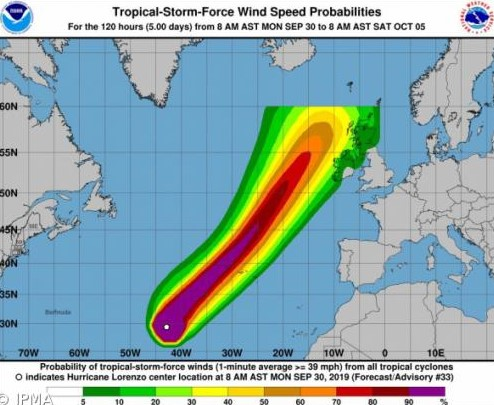
\includegraphics[width=0.4\textwidth]{Lorenzo.jpg}
    \caption{Hurricane Lorenzo}
    \label{fig:lorenzo}
\end{figure}
This paper aims to implement TETRA mobile coverage on São Miguel Island. It is intended that the region of interest has a coverage higher than 95\% of the region, serving at least 98\% of the population. It is desirable to have a similar amount of base stations of the current system. Software simulations must validate these results. The microwave links must have redundancies in order to have a functional and viable system even if there is a problem in a link.
%%%%%%%%%%%%%%%%%%%%%%%%%%%%%%%%%
\section{State of The Art And Basic Concepts Of TETRA Systems}

\subsection{State of the Art}

Public Protection and Disaster Relief Networks execute a vital role in the protection and operationality of all countries. These networks are intended to ensure communications between differents agencies, thereby ensuring interaction between all responders in emergency response. Thus, there is the possibility of producing the necessary communications between these entities at any time of the emergency\par\noindent
Hence, with resources and access to this infrastructure, it is possible to plan, coordinate, and execute the emergency plan as needed.\par\noindent
Currently, several technologies allow the implementation of this type of networks, such as:
\begin{itemize}
    \item \textbf{DMR} - Digital Mobile Radio;
    \item \textbf{dPMR} - Digital Private Mobile Radio;
    \item \textbf{LTE/PPDR} - Long Term Evolution / Public Protection and Disaster Relief;
    \item \textbf{TETRA} - Terrestrial Trunked Radio.
\end{itemize}
\par\noindent
This PPDR network is implemented with TETRA technology. Therefore, this paper describes and explains the basics of this technology. %%%%%%%%%%%%%%%%%%%%%%%
\subsection{Terrestrial Trunked Radio}
\noindent TETRA technology was standardized by ETSI and is supplied by various companies, is designed for UHF (Ultra High Frequency) voice and data transmission. TETRA has, in recent years, been the leading technology for public and private mobile radio systems, especially for public safety networks. It has been designed to have a highly stable and operational system with services that are adjustable to the needs of users. The implementation of this network can be found in most European countries (Germany, Austria, Belgium, Croatia, Finland, Greece, the Netherlands, Hungary, Ireland, Luxembourg, Norway, Portugal, Romania, Sweden, and the United Kingdom, among others).
\par\noindent
TETRA technology is a digital transmission system that uses two access methods, FDMA and TDMA. The air interface of this system is divided into carriers with different frequencies (FDMA). Each of these carriers is divided into four time-slots (TDMA). Each time-slot is a communication channel, and this factor allows each carrier to have up to four separate communications occurring at the same time.\par\noindent
Each carrier has a bandwidth of $25kHz$, linking this with the fact that there are four channels per carrier, it is possible in $200kHz$ to have thirty-two communication channels. If this technology were only built on FDMA, there would only be eight channels available in a bandwidth of  $200kHZ$. As a result of the unification of the two access methods used by TETRA, it can be said that spectrum use is very efficient and much more efficient than other technologies.
\begin{figure}
    \centering
    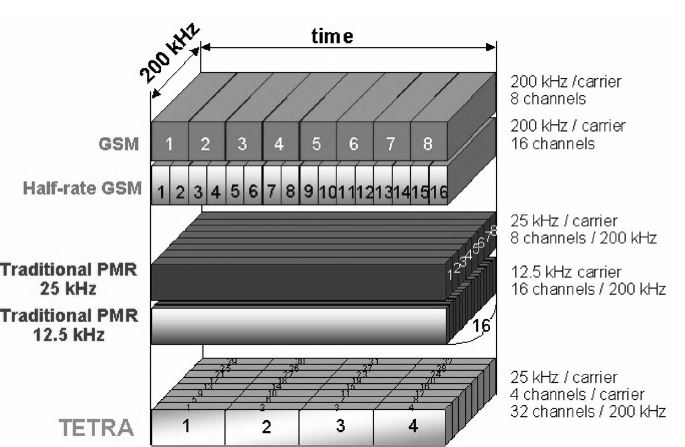
\includegraphics[width=0.45\textwidth]{TETRA_spectrum.JPG}
    \caption{Tetra spectrum usage [RETIRADO DE]}
    \label{fig:TETRAspectrum}
\end{figure}
The European Radiocommunications Committee established  the following frequency bands that this system can be operated:
\begin{itemize}
    \item  \hspace{1.2mm}   [380-385] MHz paired with [390-395] MHz for emergency services;
    \item   \hspace{1.2mm}  [385-390] MHz paired with [395-400] MHz for public services;
    \item   \hspace{1.2mm}  [410-420] MHz paired with [420-430] MHz for civil use.
\end{itemize}
\par\noindent
In PPDR  networks, it is necessary that the system easily and quickly adapts to the needs of users. To meet this need, TETRA has mechanisms and configurations that maintain system availability, allowing greater communications flexibility even during emergencies.
\par\noindent This mode also There are two main modes of operation: DMO and TMO. DMO (Direct Mode Operation) provides direct communication between two handhelds without using a base station. It can be used when the local system capacity is fully occupied or when the handheld is out of the area of coverage.\par\noindent
Besides allowing direct communications between handhelds, the Direct Mode offers the possibility of communicating through a repeater or a gateway.
\begin{itemize}
    \item \textbf{Repeater} - If two handhelds are too far apart, and out of the coverage zone of the handheld, another equipment can be configured to serve as a repeater, and therefore enables the use of direct communications.
    \item \textbf{Gateway} - It is possible to configure a mobile station to operate as a gateway. This way, this station will connect users who are out of range of the base station to the network. For example, in areas where there is no signal coverage due to terrain orography, placing one of these stations within the boundary of the base station's coverage area may be sufficient to connect users who are out of range of the base station to the network. Therefore, with this configuration, it is possible to connect the users to the control and management center.
\end{itemize}
\par\noindent Direct Mode operation is illustrated in the next figure
\begin{figure}[h]
    \centering
    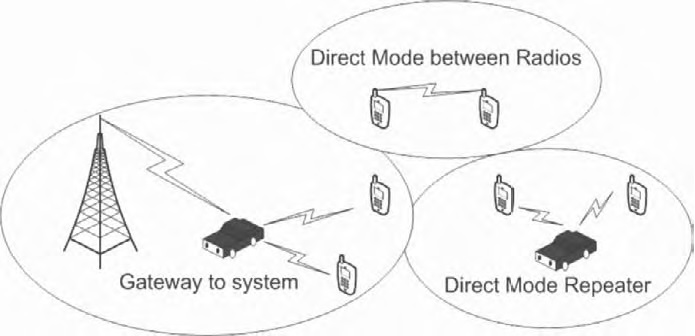
\includegraphics[width=0.45\textwidth]{DMO_PAPER.jpg}
    \caption{Direct Mode REF[]}
    \label{fig:DMO}
\end{figure}
\FloatBarrier
\subsection{SIRESP and RITERAA} 
Currently, in Portugal, the implemented PPDR network is SIRESP.  
This network was developed based on TETRA technology and was expected to cover the entire continental territory and the archipelagos.\par\noindent
It was planned that the implementation of this network would be performed in 7 distinct phases, thus guaranteeing the full functionality of this network throughout the Portuguese territory.
Currently, the SIRESP Network consists of a mobile radio coverage that ensures connection to mobile terminals, and in a fixed network.
The system has indeed reached the archipelago, but only for entities that are dependent on the state.\par\noindent
Thus, it appears that this resolution does not fit the objectives of the SIRESP network, which would be to manage all the agencies involved in security and emergency in the region.\par\noindent
The Azores Regional Civil Protection and Fire Service (SRPCBA) continued with its own communications system, but with a different operating frequency from that used in the SIRESP system. The developed system for the SRPCBA is RITERAA.
\begin{figure}
    \centering
    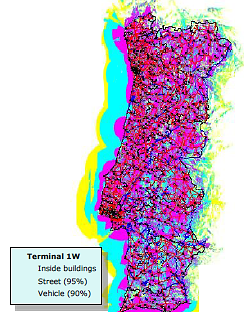
\includegraphics[width=0.35\textwidth]{SirespCobertura.png}
    \caption{S}
    \label{fig:SIRESP}
\end{figure}
\FloatBarrier
\noindent
The  Regional Government of the Azores did not accept the full implementation of the system in the archipelago. This decision was based on various factors. Those factors were financial, technical, geographical, and meteorological.\par\noindent
Another reason, provided by the responsible entities, was that the system designed to operate in the Azores paid no particular attention to the terrain orography neither to the natural geographical discontinuity of the archipelago. This factor could lead to a lack of coverage in some regions. Also, the implementation of  SIRESP would not be the most suitable for making connections between the islands of the archipelago.\par\noindent
RITERAA was developed in 2014. Instead of TETRA, this network uses DMR technology. RITERAA allows reaching coverage of $ 95 \% $ of the Azorean territory, reaching $ 98 \% $ of the population, thus allowing greater efficiency and reliability in communications. São Miguel Island has eleven base station. The localization of these base station are shown in the next figure. 
\begin{figure}[h]
    \centering
    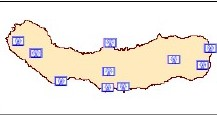
\includegraphics[width=0.45\textwidth]{riteraaestacoesbase.jpg}
    \caption{Localization of the base stations in São Miguel Island}
    \label{fig:RITERAA}
\end{figure}
\FloatBarrier
%%%%%%%%%
\section{Fundamental Concepts}
In problems of mobile coverage, it is decided to place the base station in order to optimize coverage. In mobile communications, it is intended that the range of the base station does not exceed a particular limit. This area with defined limits is called the cell.\par\noindent 
The design of the cell, in which the size is pre-established, takes into account the
telecommunications traffic aspects, quality of service, and propagation aspects.\par\noindent
The variability of the received signal depends on the type of cell in which the mobile terminal is located.\par\noindent
In mobile coverage, the cell can be defined in three different types:
\begin{itemize}
    \item Macro cell;
    \item Micro cell;
    \item Pico cell;
\end{itemize}
The designation of the cell it's not correlated with the size of the cell. It's related to the Line-of-Sight situation.\par\noindent
Macro-cells are defined as coverage areas where there is no line-of-sight between the base station and mobile terminals. The base station antennas are usually above the tops of buildings, while mobile terminals are generally in shadowed areas of obstacles.\par\noindent 
The micro cell is a coverage region where the mobile terminal is usually in line-of-sight with the base station. The base station antenna is usually below the tops of buildings. For example, the cell is a street and the fixed terminal is placed on a light pole, with this configuration is intended to cover the length of the street.
\begin{figure}[h]
    \centering
    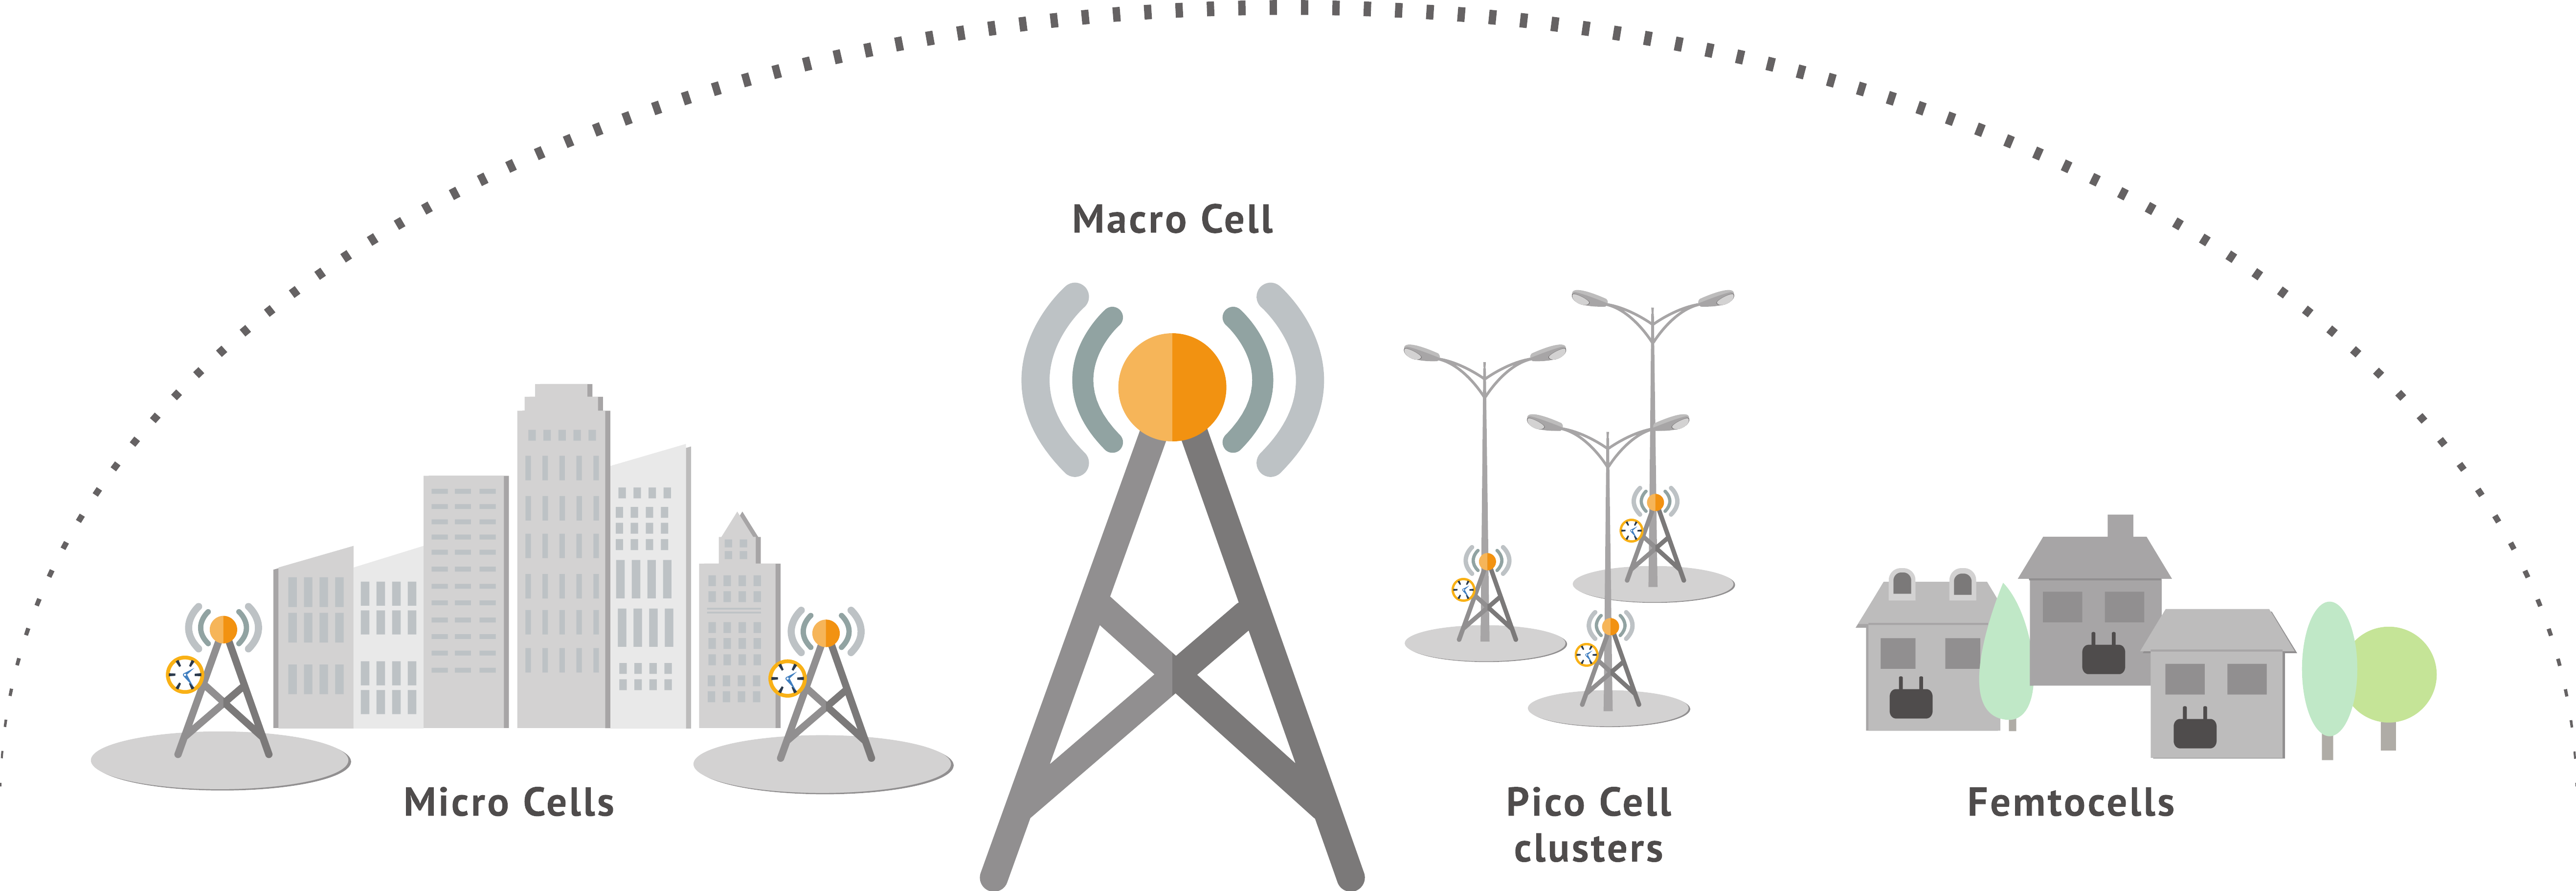
\includegraphics[width=0.45\textwidth]{celulas.png}
    \caption{Cells []}
    \label{fig:celulas}
\end{figure}
\FloatBarrier
Since this paper aims to design a PPDR network and this type of network is usually associated with outdoor propagation, the macro cell is the predominant type of cell. 
%%%%%
\subsection{Fading}
In mobile communications, fading can be described as the received signal variation over a certain period. This fluctuation in the level of the received signals, and consequently, the disturbance of the quality of service, is caused by the variability (in time) of the electromagnetic wave propagation medium characteristics.
\begin{figure}[h]
    \centering
    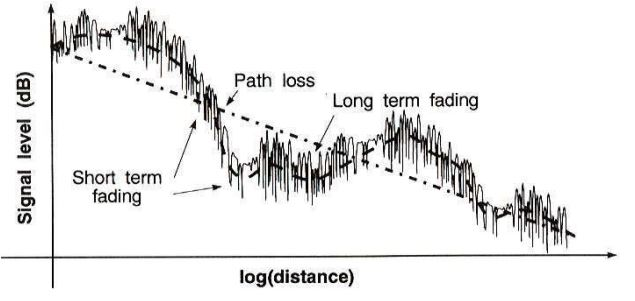
\includegraphics[width=0.45\textwidth]{fading.JPG}
    \caption{Signal Variation}
    \label{fig:fading}
\end{figure}
\par\noindent
There are two types of fading, slow fading and fast fading. Fast variations in the received signal characterize fast fading. On the other hand, slow fading is characterized by a variation in the received signal with a very long duration (minutes or even hours).
\par\noindent Fast fading is mainly caused by the multipath of the signal and can be interpreted as local turbulence of the atmosphere, resulting predominantly from two factors: frequency of operation and the location of the antennas. There is multipath when it is possible to establish more than one distinct path between the base station and the terminal. These distinct paths may give rise to interference at the terminal since they are two signals with similar amplitudes and relative phase dependent on the path.\par\noindent Fading is a random phenomenon. Thus, it results from random processes and can be approximated by statistics.\par\noindent
Since this paper is focused on outdoor propagation, the most common situations will be non-line-of-sight. Therefore, to characterize the fading, it is used the Rayleigh Distribution.  This distribution is associated with a fast variation of the signal. 

\subsection{Diversity}
It is not always economical, or technically possible, to increase the transmitted power or antenna gain so that the received power is higher than the receiver's sensitivity. Thus, to mitigate the effects of fading, diversity is often used.
This technique is mainly used to prevent the effects of fast fading. It consists of using the redundancies of the signals at the reception. The use of diversity is usually associated with signal combination.
\par\noindent
Diversity can be divided into several types, but there are two that are often used:
\begin{itemize}
    \item \textbf{Spatial Diversity} - The signals received by the base station antennas are the result of wave propagation through multipath. Multiple spaced antennas are used to receive the signal transmitted by handheld.Typically the antenna spacing is horizontal.
    \item\textbf{Frequency Diversity} - Frequency diversity is based on the multiple transmission of signals at different frequencies. In this way, the antennas receive the same signal but with different operating frequencies. In this type of diversity, larger bandwidth is required.
\end{itemize}
\subsection{Combining}
The use of diversity requires a combinator at the reception. When in a path the received signal is obtained through $ n $ uncorrelated signals, the diversity used is of the order $ n $. Given the diversity order, the matching process is to get a better signal than any of the existing $ n $ signals, or at least, equal to the best of these signals.\par\noindent
The combining process used in this project was the selection. The combination by selection is based on the choice of the best-transmitted signal . That is, the signal that is selected for the combiner output is at all times the most intense received signal. Since the fading is charactherized by the Rayleigh Distribution, the combining values are also extracted from the Rayleigh Distribution for $n$ uncorrelated signals. 
\begin{figure}[h]
    \centering
    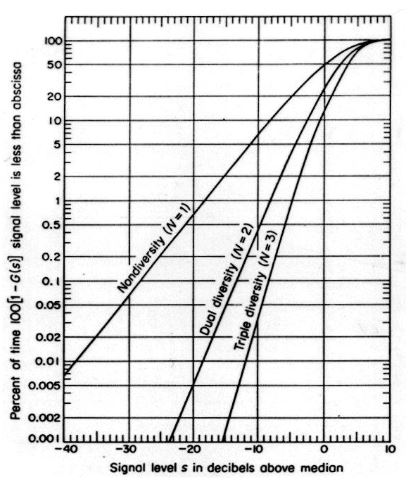
\includegraphics[width=0.285\textwidth]{combinacaoRayleigh.jpg}
    \caption{Combining by selection}
    \label{fig:combining}
\end{figure} \FloatBarrier
\subsection{Propagations Model}
In mobile coverage implementation, due to coverage and interference reasons, it is necessary to estimate the signal transmitted by the base station. A good estimate of the signal received at the cell boundary is required.\par\noindent
To estimate the signal one must use propagation models. Most of these models provide the mean or median value of the signal. 
Before applying the propagation models, it is necessary to classify the area under study. Typically, study zones are divided into three different categories:
\begin {itemize}
    \item \textbf{Urban area} - zone of high construction density, with large building blocks and towers, usually with more than two floors per building;
    \item \textbf{Suburban area} - residential area, lower volume buildings with gardens and parks. It is a not very dense zone around the mobile terminal;
    \item \textbf{Rural area}- open areas, a few buildings. There are usually no obstacles between 300-400m around the mobile terminal.
\end {itemize} \par\noindent
Before the propagation  models are introduced, it is necessary to present a set of characteristics of the outdoor environments in mobile radio.
\begin {enumerate}
    \item The mobile terminal antenna is typically at the height of $ 1.8 $ meters from the ground;
    \item Even if the route analyzed is a LoS situation, there is a possibility that there are zones nearby where this situation does not occur;
\end {enumerate}
The models used in macro-cell scenarios can be summarized into two essential models:
    \begin{itemize}
        \item \textbf{Okumura-Hata}: Distances greater than $ 5km $ (Urban, Suburban, Rural);
        \item \textbf{Walfish-Ikegami}: Distances under $ 5km $ (Urban and Suburban Environments);
    \end{itemize}
%%%%%%
\subsection{Okumura-Hata}
This empirical model was first introduced in 1968 by Okumura. It was based on measurements made in the frequency spectrum between $ 150 MHz $ and $ 2000 MHz $. Through the proposed graphical representations, Hata in 1980 established the equations that best fit the graphical representation.\par\noindent
This model gives the average value of path attenuation. It depends on frequency ($ f $), the distance between the base station and mobile terminal ($ d $) and antenna height of the mobile terminal ($ h_m $).\par\noindent
Following the Hata's reformulation, this model is valid under the conditions of the table.
\begin{table}[h]
\centering
\begin{tabular}{|c|c|c|ll}
\cline{1-3}
            & Minimal Value & Maximum Value &  &  \\ \cline{1-3}
$f [MHz] $  & 150             & 1500            &  &  \\ \cline{1-3}
$d [km]$    & 1               & 20              &  &  \\ \cline{1-3}
$h_{be}[m]$ & 30              & 200             &  &  \\ \cline{1-3}
$h_m [m]$   & 1               & 10              &  &  \\ \cline{1-3}
\end{tabular}
\caption{Valid values for Okumura-Hata Model}
\label{tab:validadeHATA}
\end{table}
The median value of the pathloss is given by the next expression.
\begin{equation} \label{equation:Lpokumurahata}
\begin{split}
    L_p [dB] = 69.55+26.16\log(f_{[MHz]})-13.82\log(h_{be[m]})\\+[44.9
    0-6.55\log(h_{be[m]})]\log(d_{[km]})\\-H_{mu[dB]}(hm,f)- \sum Correction Factors
\end{split}
\end{equation}
\par\noindent
 $H_{mu[dB]}$ and th correction factors can be determined with the formulas from \cite{c1}. 
In the Okumura-Hata model $ h_ {be} $ can be calculated by:
\begin{equation}
    \label{equation: hbeOkhata}
    h_ {be [m]} = h_ {bs [m]} - h_ {ga [m]}
\end{equation}
\begin{itemize}
    \item[] $ h_ {be [m]} $ - Effective height of base station antenna;
    \item[] $ h_ {bs [m]} $ - Total height of base station antenna (sum of mast height plus terrain elevation);
    \item[] $ h_ {ga [m]} $ - Average land height value.
\end{itemize}
$h_ {ga [m]}$ is the average terrain height between 3km to 15km. This condition is valid for paths that reach a distance of  15km or greater. In circumstances where the distance is less than 15km, and terrain information is available, the average terrain height should be between $ 0.2d $ to $d$.
%%%%
\subsection{Walfisch-Ikegami}\par \noindent
The \textit{Walfisch-Ikegami} model adapts the \textit{Ikegami} and \textit{Walfisch-Bertoni} models. That is, it assumes the propagation conditions of the \textit{Walfisch-Bertoni} model, but the propagation considered between the diffraction edge of the building and the mobile terminal is adapted from \textit{Ikegami}.
\begin{figure}[h]
    \centering
    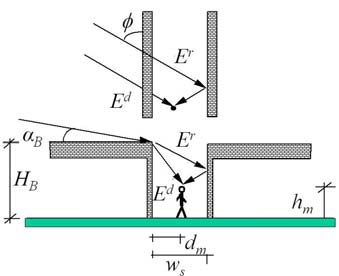
\includegraphics[width=0.45\textwidth]{Wbertoni_efeitomultipercurso.jpg}
    \caption{Multipath}
    \label{fig:multipercurso}
\end{figure}
\begin{figure}[h]
    \centering
    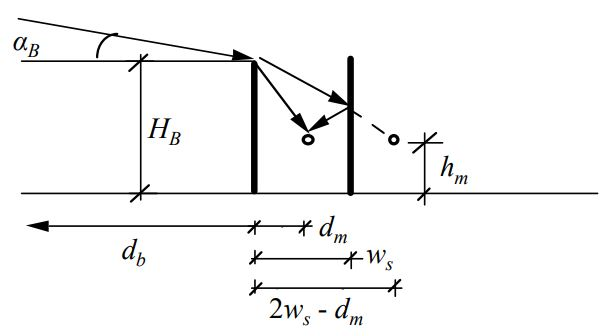
\includegraphics[width=0.45\textwidth]{Ikegami.JPG}
    \caption{Building refraction}
    \label{fig:ikegami}
\end{figure}
If the handheld and the base station are in a line-of-sight situation ($\Phi=0$), then the formula to calculate the median path loss is:
\begin{equation}
    L_{p[dB]}=42.6+26\log(d_{[Km]})+20\log(f_{[MHz]}),d>0.02Km
\end{equation}\par\noindent
In all other cases, the expression that must be applied is:
\begin{equation}
    L_{p[dB]}=
        \begin{cases}
        L_{0[dB]}+L_{rt[dB]}+L_{rm[dB]}, & \text{$L_{rt}+L_{rm}>0$}\\
        L_{0[dB]}, &\text{$L_{rt}+L_{rm}\leq0$}
        \end{cases}
\end{equation}\par\noindent
$L_{rt}\ \textrm{e}\  L_{rm}$ can be defined as:
\begin{equation}\label{equation:walfisch_ikegami_lrm}
\begin{split}
    L_{rm[dB]}=-16.9-10\log(w_{s[m]})+10\log(f_{[MHz]})+\\+20\log(H_{B[m]}-h_{m[m]})+L_{ori[dB]}
\end{split}
\end{equation}
\begin{equation}
\begin{split}
    L_{rt[dB]}=L_{bsh[dB]}+k_a+k_d\log(d_{[Km]})+\\+k_f\log(f_{[MHz]})-9\log(w_{B[m]})
\end{split}
\end{equation}\par\noindent
The correction factors ($k_a,\ k_d, \ k_d$) can be consulted in \cite{c1}.\par\noindent
The validity conditions of this model can be viewed in the next table.
\begin{table}[h]
\centering
\begin{tabular}{|c|c|c|ll}
\cline{1-3}
            & Minimal Value & Maximum Value &  &  \\ \cline{1-3}
$f [MHz] $  & 800             & 2000            &  &  \\ \cline{1-3}
$d [km]$    & 0.02               & 5              &  &  \\ \cline{1-3}
$h_{be}[m]$ & 4              & 50             &  &  \\ \cline{1-3}
$h_m [m]$   & 1               & 3              &  &  \\ \cline{1-3}
\end{tabular}
\caption{Validity conditions of Walfisch-Ikegami model}
\label{tab:validade_walsfisch-ikegami}
\end{table}
%%%%%
\section{Coverage Design}
\subsection{Antennas}\noindent
To design the mobile coverage, one must take into account what antennas are going to be used. In this paper, the focus is aimed at sectorized antennas.
\par\noindent
Sectorized antennas have a smaller beamwidth. Hence they have a higher gain value. The horizontal radiation pattern has a half-power beamwidth of 120 degrees. Sectorization has some advantages, such as co-channel interference reduction, reduced frequency reuse distance, high antenna gain. \par\noindent
Each sector can be viewed as a cell, allowing each antenna to be adjusted according to the sector's needs (\textit{downtilt}, emitted power, diversity, antenna height).\par\noindent
The antenna used in this paper has a gain of 11.5 dBi.
\begin{figure}[h]
    \centering
    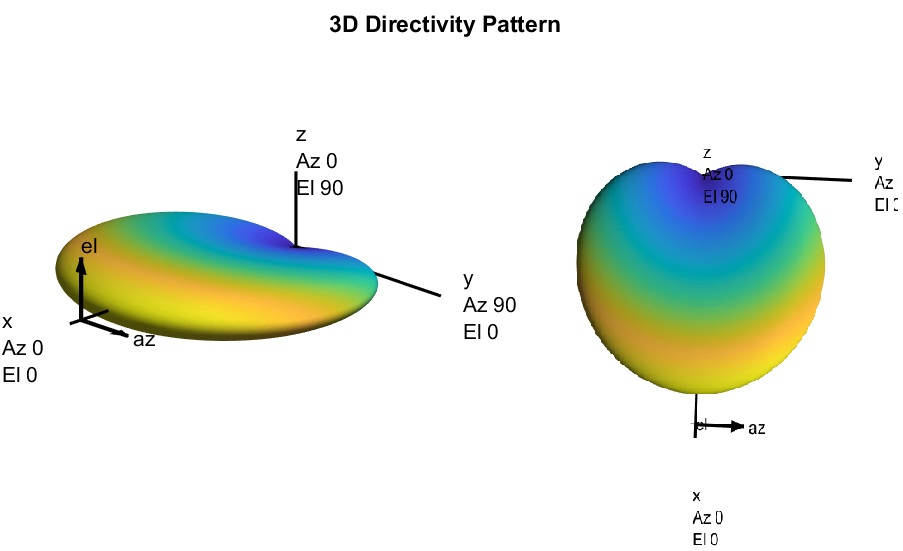
\includegraphics[width=0.45\textwidth]{antenasectorizada.JPG}
    \caption{Sectorized Antenna}
    \label{fig:antenna3D}
\end{figure}
\FloatBarrier
%%%%%%
\subsection{Sensivity and Considered Attenuation}\noindent
One can define sensitivity as the minimum value of the signal that the receiver's antenna can detect the transmitted information. The restrictive factor of the maximum range of the connection between the base station mobile terminal is the uplink connection.  Therefore, the receiver sensitivity in uplink is the base station sensitivity value. In this case, the sensitivity value of the base station is  -113.5dBm. \par\noindent
The considered handheld sensitivity value was -103dBm. This value corresponds to a mobile terminal in a dynamic state. \par\noindent
Despite having the sensitivity values of the equipment, one must consider other types of attenuation. In PPDR networks, it must be considered the fire attenuation, user attenuation and the vegetation attenuation. The assumed values were:
\begin{itemize}
    \item \textbf{Fire Attenuation}- 15 dB;
    \item \textbf{User Attenuation}- 5dB;
    \item \textbf{Vegetation Attenuation}- Weissberger Model\cite{c1}.
\end{itemize}
\par\noindent
Even after all this considerations, it is possible to appear in the project some areas with no coverage, because of this assumption, it was added a safety margin of 10 dB.
\subsection{Cell Design} \noindent
In total it was designed eleven base station. Each base section has two or three sectors. This process is very extensive and detailed, because of this, it is not possible to describe it in this paper. Therefore, only the final values will be presented. 
\begin{figure}[h]
    \centering
    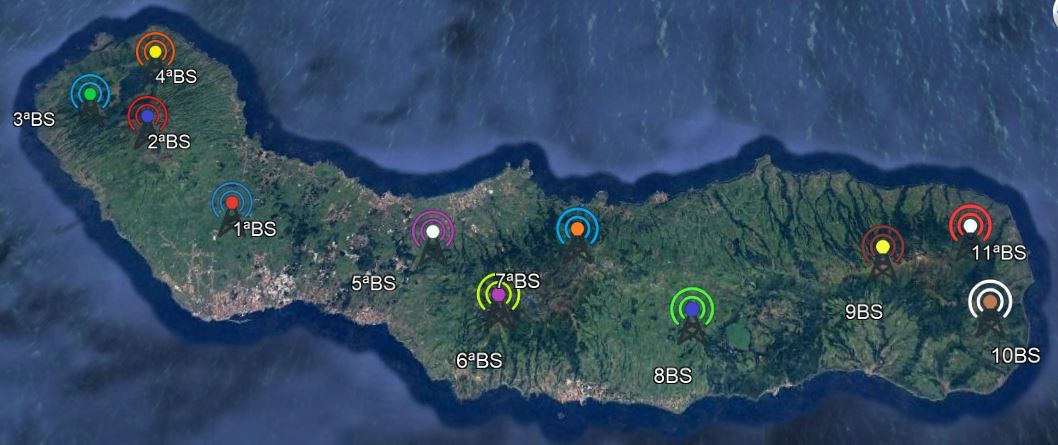
\includegraphics[width=0.49\textwidth]{localizacaoBS.JPG}
    \caption{Location of the Implemented Base Stations}
    \label{fig:my_label}
\end{figure}
\par\noindent
In total there are thirty sectors. The summarized information about these sector can be found in the next table.
\begin{table}[h]
\centering
\begin{tabular}{|c|c|c|c|}
\hline
\rowcolor[HTML]{EFEFEF} 
{\color[HTML]{000000} \textbf{Base Station}} & \multicolumn{3}{c|}{\cellcolor[HTML]{EFEFEF}{\color[HTML]{000000} \textbf{Transmitted Power (W)}}}     \\ \hline
                                             & \cellcolor[HTML]{FD6864}Sector 1 & \cellcolor[HTML]{96FFFB}Sector 2 & \cellcolor[HTML]{FFFE65}Sector 3 \\ \hline
\textbf{1st}                                 & 119.95                           & 65.17                            & 65.46                            \\ \hline
\textbf{2nd}                                 & 119.4                            & 58.21                            & —                                \\ \hline
\textbf{3rd}                                 & 63.97                            & 23.28                            & 19.41                            \\ \hline
\textbf{4th}                                 & 10.31                            & 22.65                            & 37.93                            \\ \hline
\textbf{5th}                                 & 114.03                           & 54.33                            & 208.45                           \\ \hline
\textbf{6th}                                 & 25.53                            & 52.73                            & —                                \\ \hline
\textbf{7th}                                 & 19.18                            & 26.49                            & —                                \\ \hline
\textbf{8th}                                 & 116.15                           & 1.982                            & 104.23                           \\ \hline
\textbf{9th}                                 & 68.55                            & 241.55                           & 83.56                            \\ \hline
\textbf{10th}                                & 11.17                            & 7.23                             & 6.68                             \\ \hline
\textbf{11th}                                & 115.35                           & 27.92                            & 156.32                           \\ \hline
\end{tabular}
\caption{Parameters of the Base stations}
\label{tab:BS}
\end{table}\par\noindent 
There is a zone is this project that was not dimensioned to be covered.  This zone is called Lagoa do Fogo. The reason for this approach is simple. Lagoa do Fogo is one of the highest points of the island, very irregular terrain and with no human occupation. Therefore, this area was not accommodated in the project.
\subsection{Transportation Network}
\noindent
A telecommunications network is an aggregate of nodes and links and is used to carry information between different devices. Usually, these equipment are separated by dozens of kilometres. This transport of information must be done efficiently. Network nodes, also known as network elements, correspond to electronic or optical devices (computers, switches, routers, multiplexers) that originate, guide, or terminate information.\par\noindent
In the case of this network, it will be used microwave links. Microwave links have two significant advantages. The first advantage is that they are immune to fire attenuation, communications are only damaged if base stations are damaged by fire. The second advantage is that it is not necessary to use a physical medium (coaxial cable or optical fiber). Since base stations are in remote locations it would be expensive to interconnect them by a physical medium.\par\noindent
The established network can be seen in the next figure.
\begin{figure}[h]
    \centering
    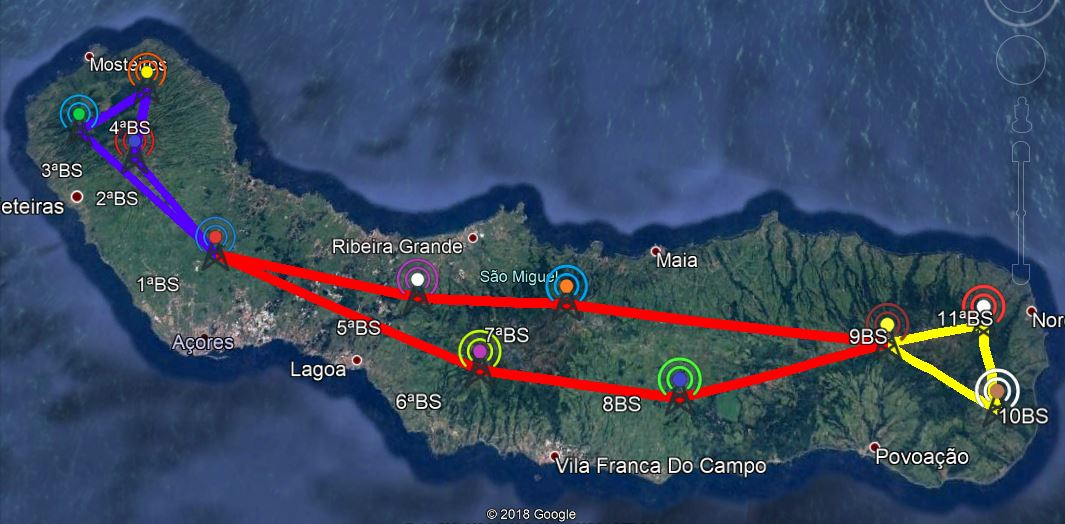
\includegraphics[width=0.45\textwidth]{RedeEB.JPG}
    \caption{Network Topology}
    \label{fig:topologia}
\end{figure}
\FloatBarrier

\noindent The physical topology is a ring topology. As three rings are interconnected, the correct designation is a triple ring network. This topology introduces redundancies in the network, in case of failure of one of the links, it is possible to continue to communicate with other base stations.
\par\noindent
The logical topology is of this network is a star topology. 
\begin{figure}
    \centering
    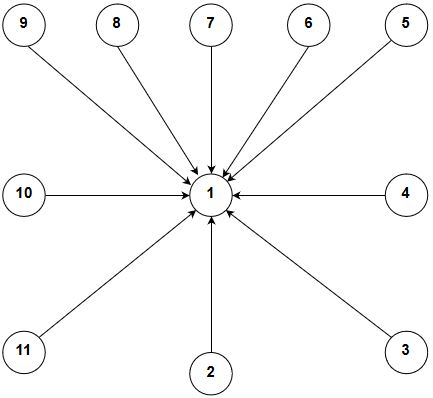
\includegraphics[width=0.45\textwidth]{topologicarede.JPG}
    \caption{Logical Topology}
    \label{fig:logical}
\end{figure}
\section{Simulations}\noindent
Simulations were done in order to validate the design of mobile coverage.\par
\noindent Therefore, four different scenarios were simulated.
\subsection{Dynamic Receiver with Fire Attenuation}
\noindent This is the worst-case scenario. Also, it is the rarest case. This approach is done by simulating that there are fire near to the base stations. Despite having this attenuation it is expected a good coverage.
\begin{figure}[h!]
    \centering
    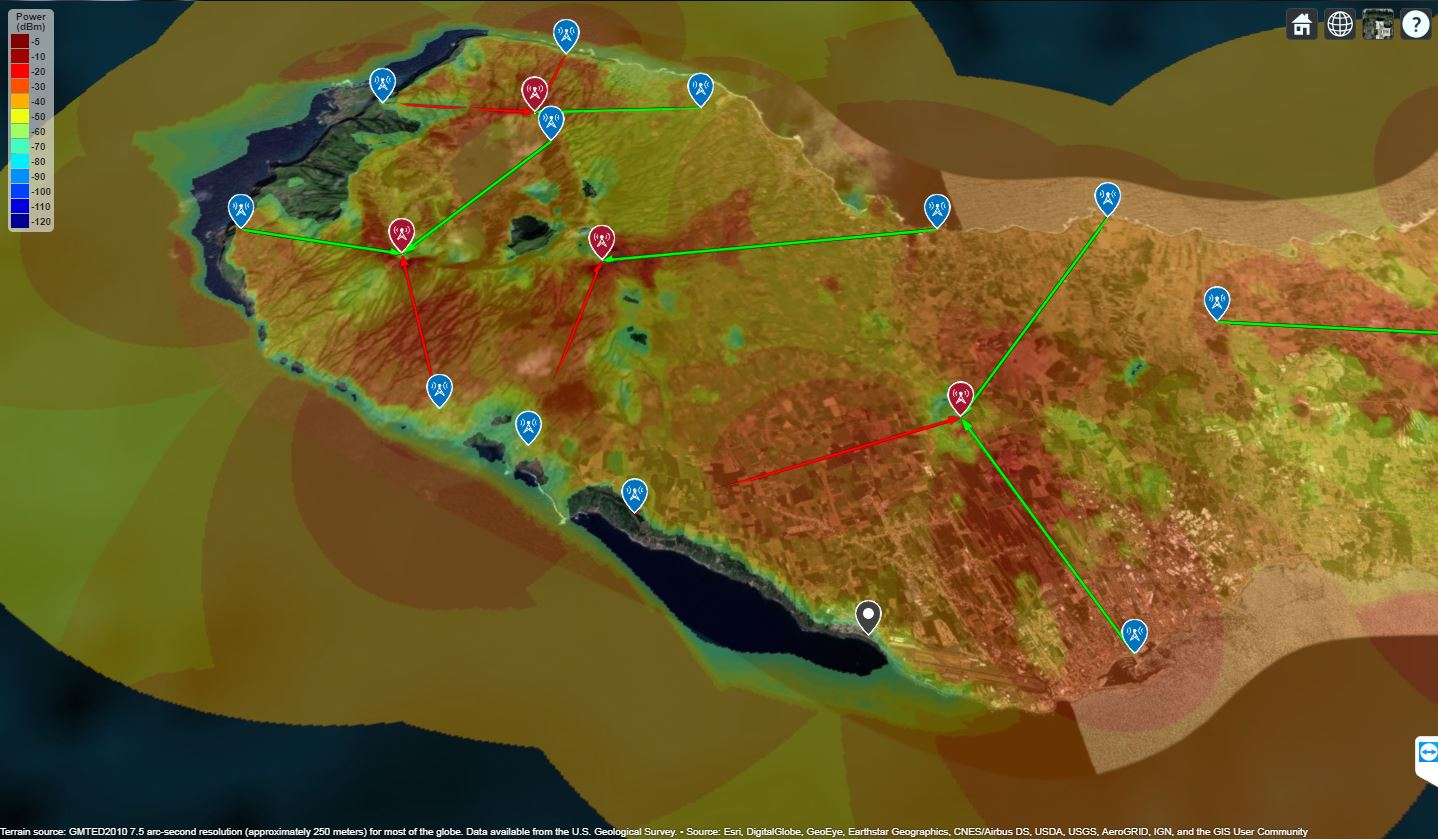
\includegraphics[width=0.45\textwidth]{estacaobase1a4.JPG}
    \caption{Base Station 1 to 4}
    \label{fig:estacoesbase1a4}
\end{figure}
\begin{figure}[h!]
    \centering
    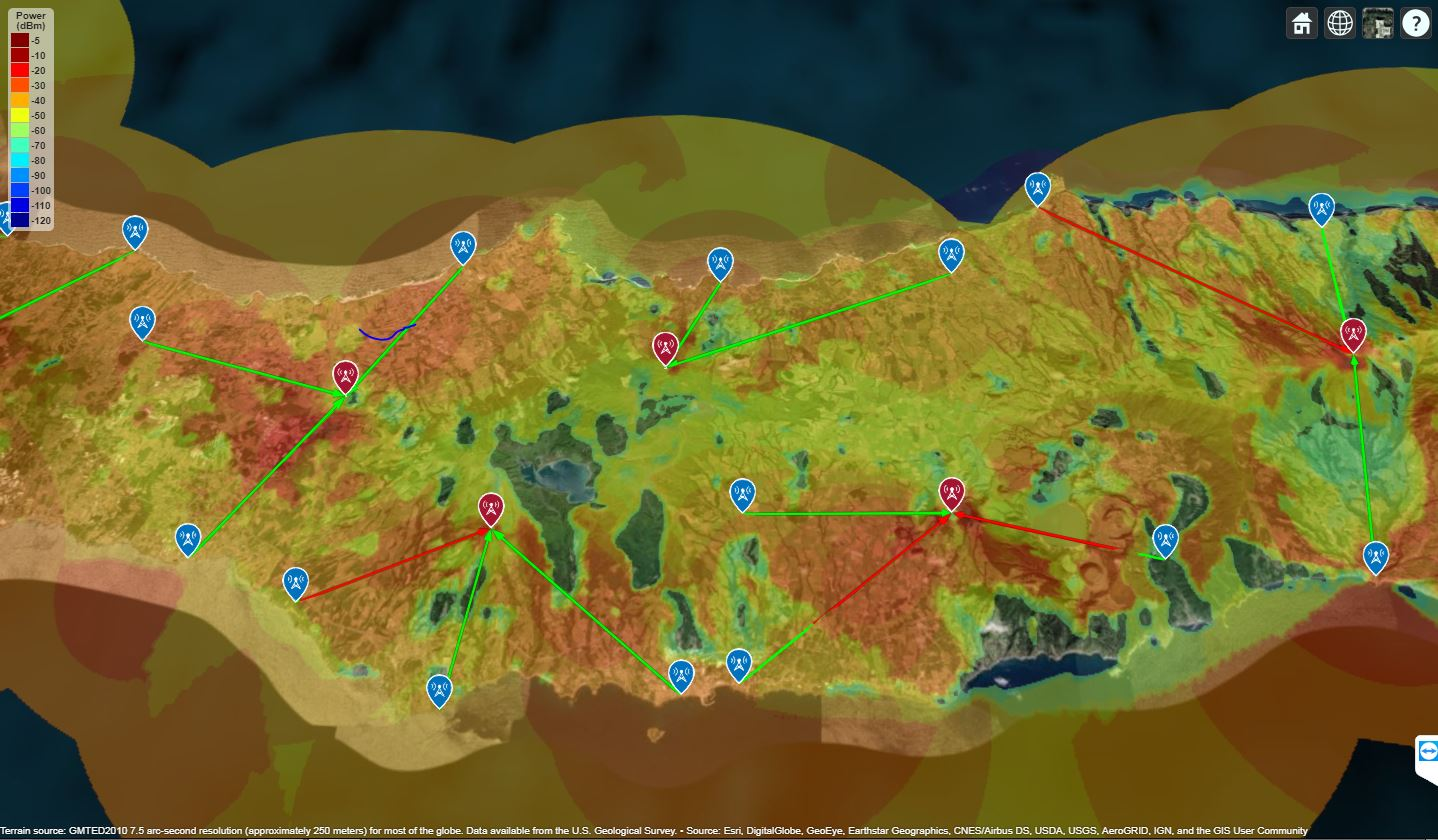
\includegraphics[width=0.45\textwidth]{estacaobase5a8.JPG}
    \caption{Base Station 5 to 8}
    \label{fig:estacoesbase5a8}
\end{figure}
\begin{figure}[!h]
    \centering
    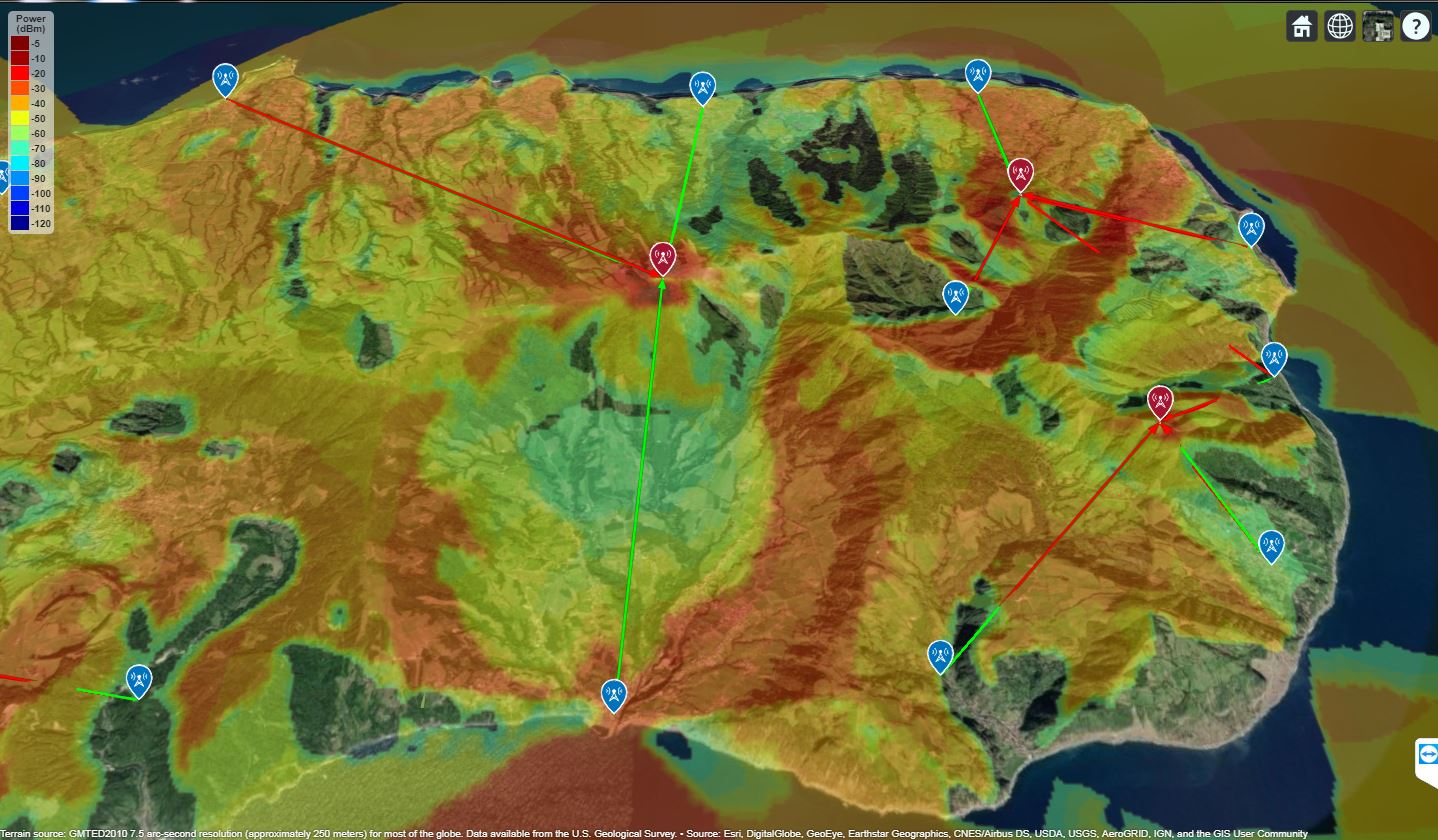
\includegraphics[width=0.45\textwidth]{estacaobase9a11.JPG}
    \caption{Base Station 8 to 11}
    \label{fig:estacoesbase9a11}
\end{figure}
\FloatBarrier 
\noindent As one can see in the figures above, all the suburbans areas are covered. Therefore, the zones with higher population density are covered by this network. Figure \ref{fig:estacoesbase9a11} has the most number of areas without coverage. These are rural areas. There is no human occupation in those areas. It is possible to affirm that this network satisfies the main goals.
\subsection{Static Receiver with Fire Attenuation}\noindent
In this scenario, the handheld has a sensitivity 10dB lower than the previous case. This value has a huge impact on coverage levels.
\begin{figure}[h!]
    \centering
    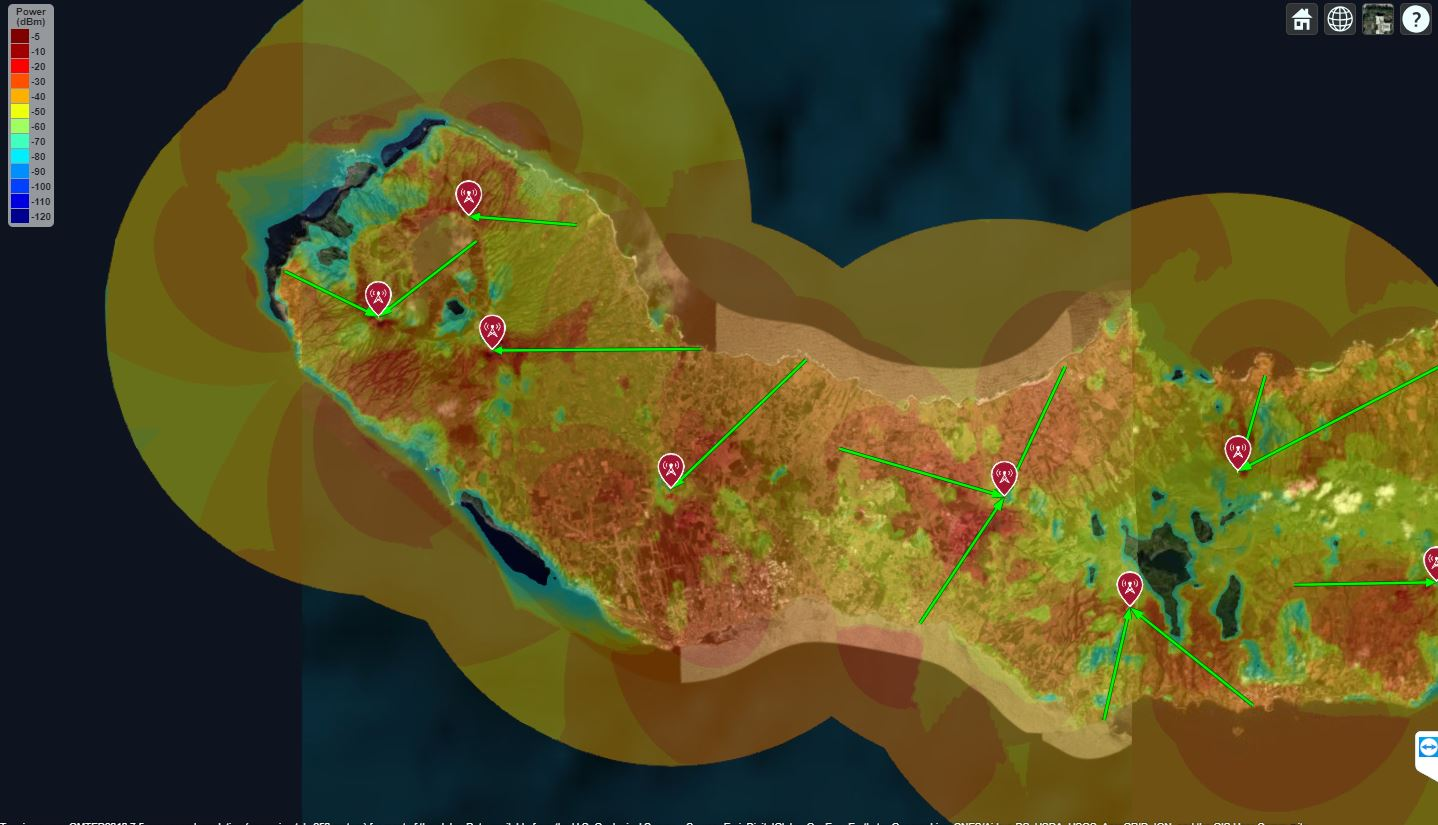
\includegraphics[width=0.45\textwidth]{esteEstatico.JPG}
    \caption{Coverage for a static receiver - I}
    \label{fig:estaticoESTE}
\end{figure}
\begin{figure}[h!]
    \centering
    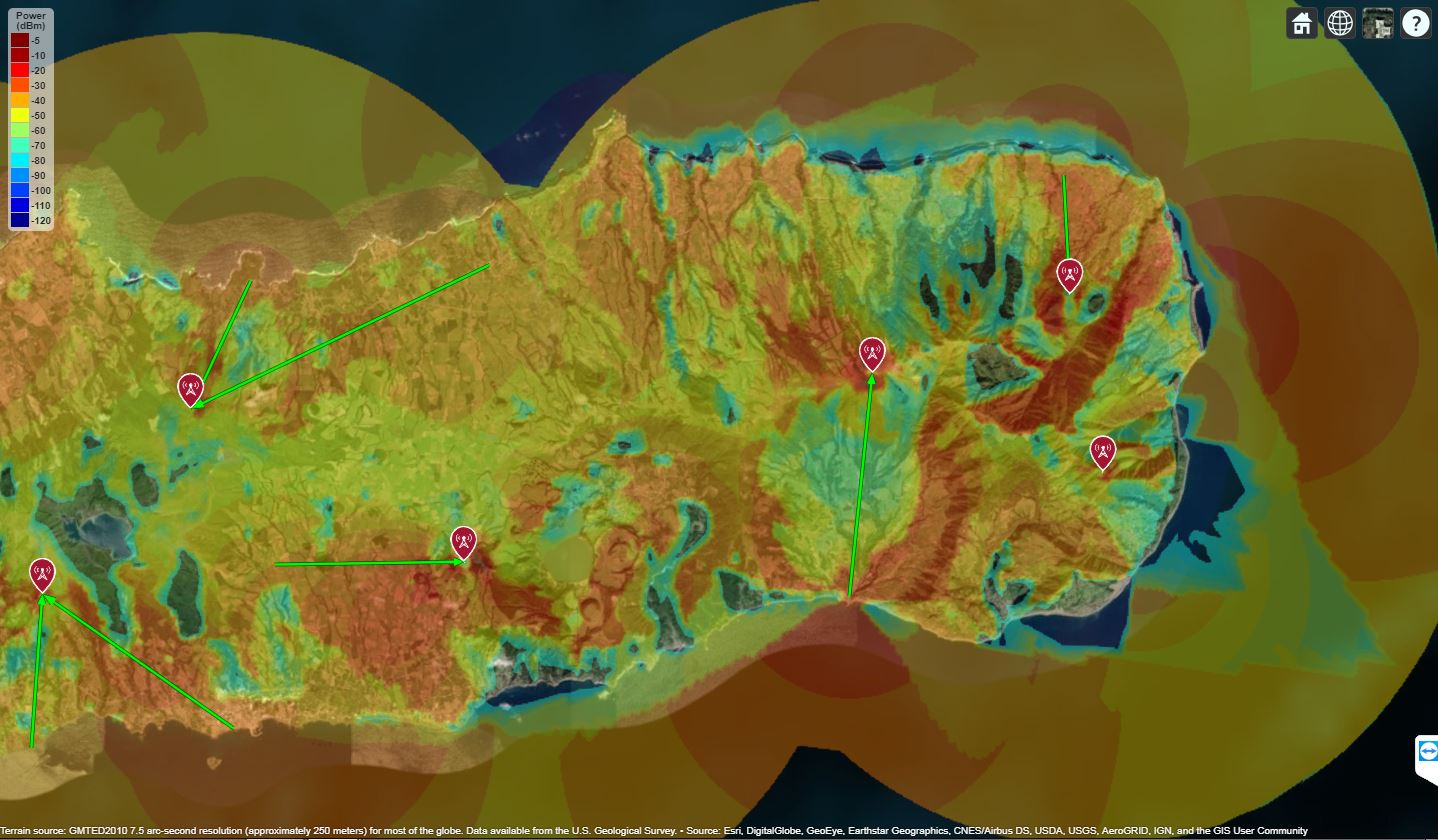
\includegraphics[width=0.45\textwidth]{OesteEstatico.JPG}
    \caption{Coverage for a static receiver - II}
    \label{fig:estaticoOeste}
\end{figure} \FloatBarrier
\subsection{Dynamic Receiver without Fire Attenuation}\noindent
In this case, the handheld is in a dynamic state, but the signal is not attenuated by fire. This situation has a minimal received signal 15dB lower than the first scenario. 
\begin{figure}[h!]
    \centering
    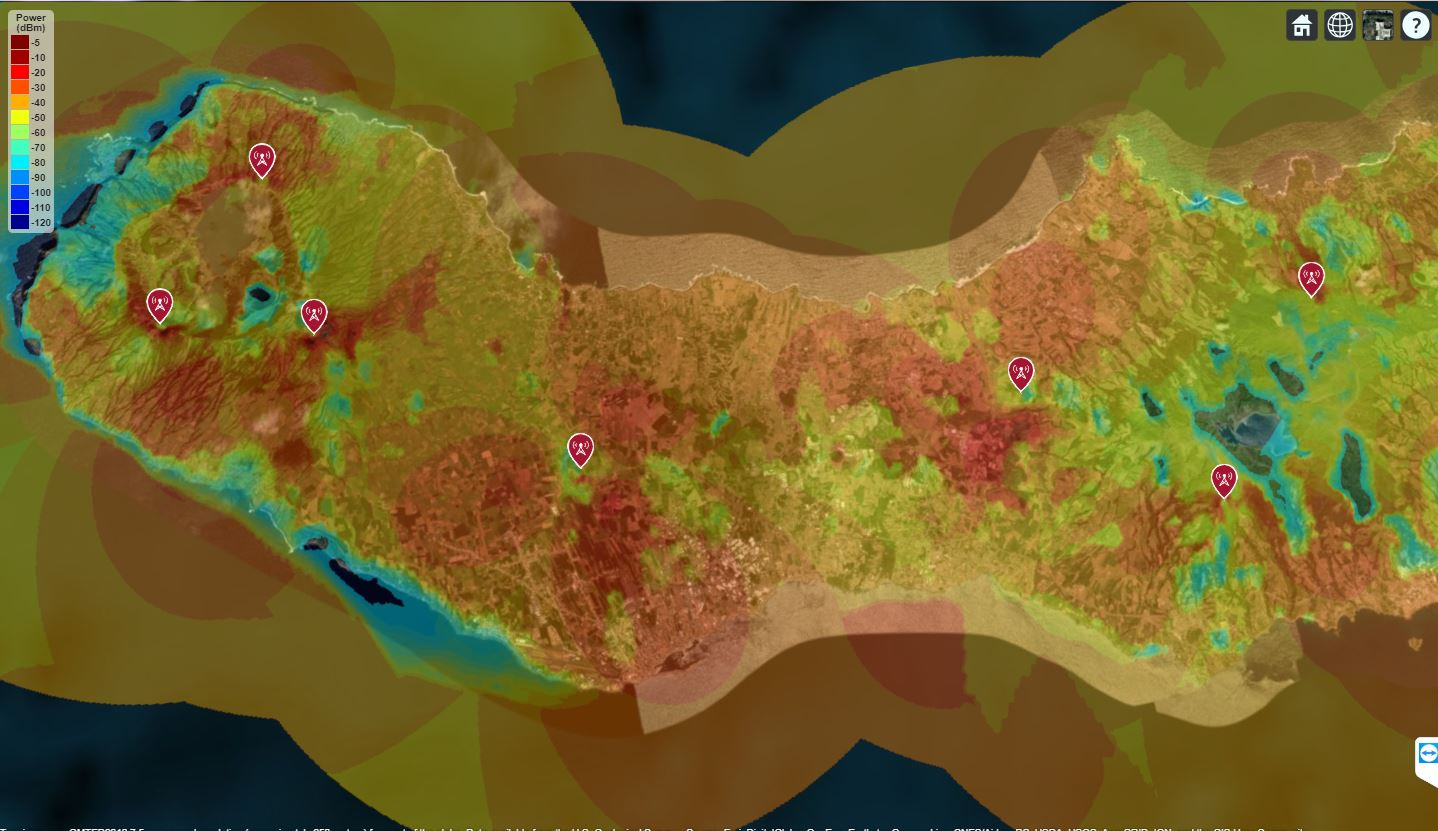
\includegraphics[width=0.45\textwidth]{RecetorDinamicoSemfogoI.JPG}
    \caption{Coverage for a dynamic receiver without fire attenuation - I}
    \label{fig:dinamicosemfogESTE}
\end{figure}
\begin{figure}[h!]
    \centering
    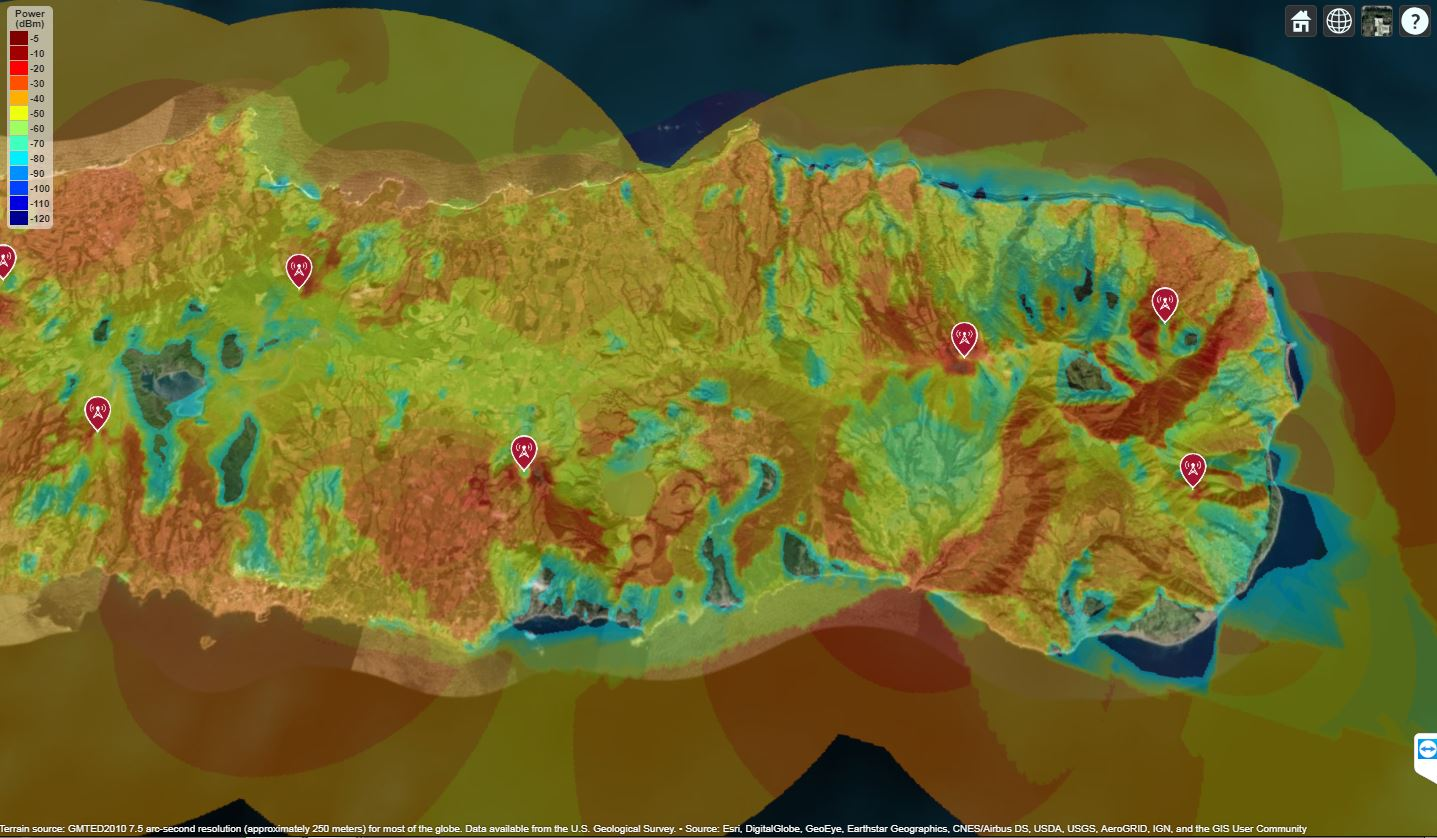
\includegraphics[width=0.45\textwidth]{RecetorDinamicoSemfogoII.JPG}
    \caption{Coverage for a dynamic receiver without fire attenuation - II}
    \label{fig:dinamicosemfogoOeste}
\end{figure} \FloatBarrier
\noindent
In this scenario, one can see that almost all the island is covered by this network.
\subsection{Static Receiver without Fire Attenuation}
\noindent This scenario is the best-case scenario. The worst-case scenario has an extra attenuation of 15dB when compared with this scenario.
\begin{figure}[h!]
    \centering
    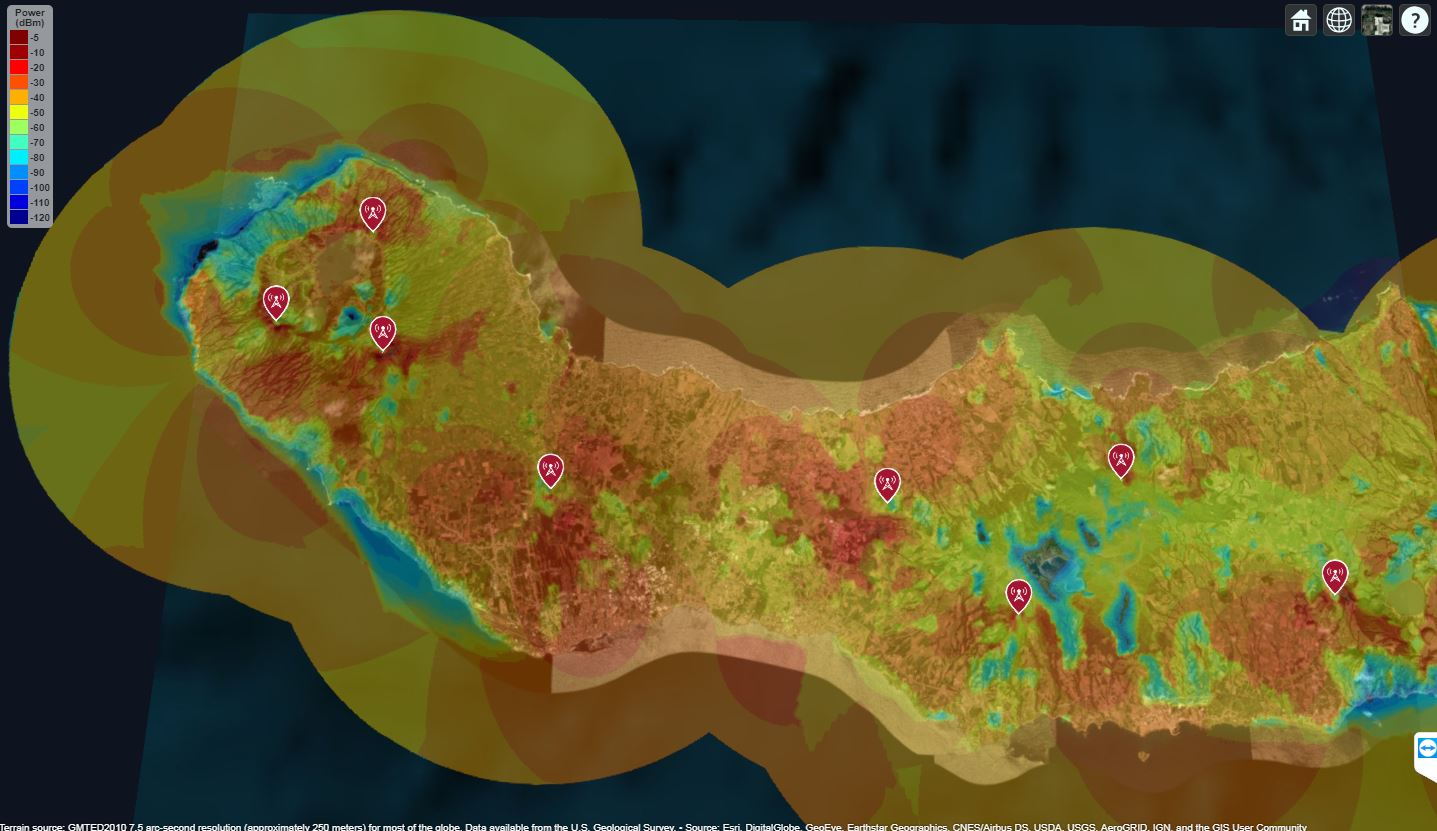
\includegraphics[width=0.45\textwidth]{RecetorEstaticoSemfogoI.JPG}
    \caption{Coverage for a static receiver without fire attenuation - I}
    \label{fig:estaticosemfogESTE}
\end{figure}
\begin{figure}[h!]
    \centering
    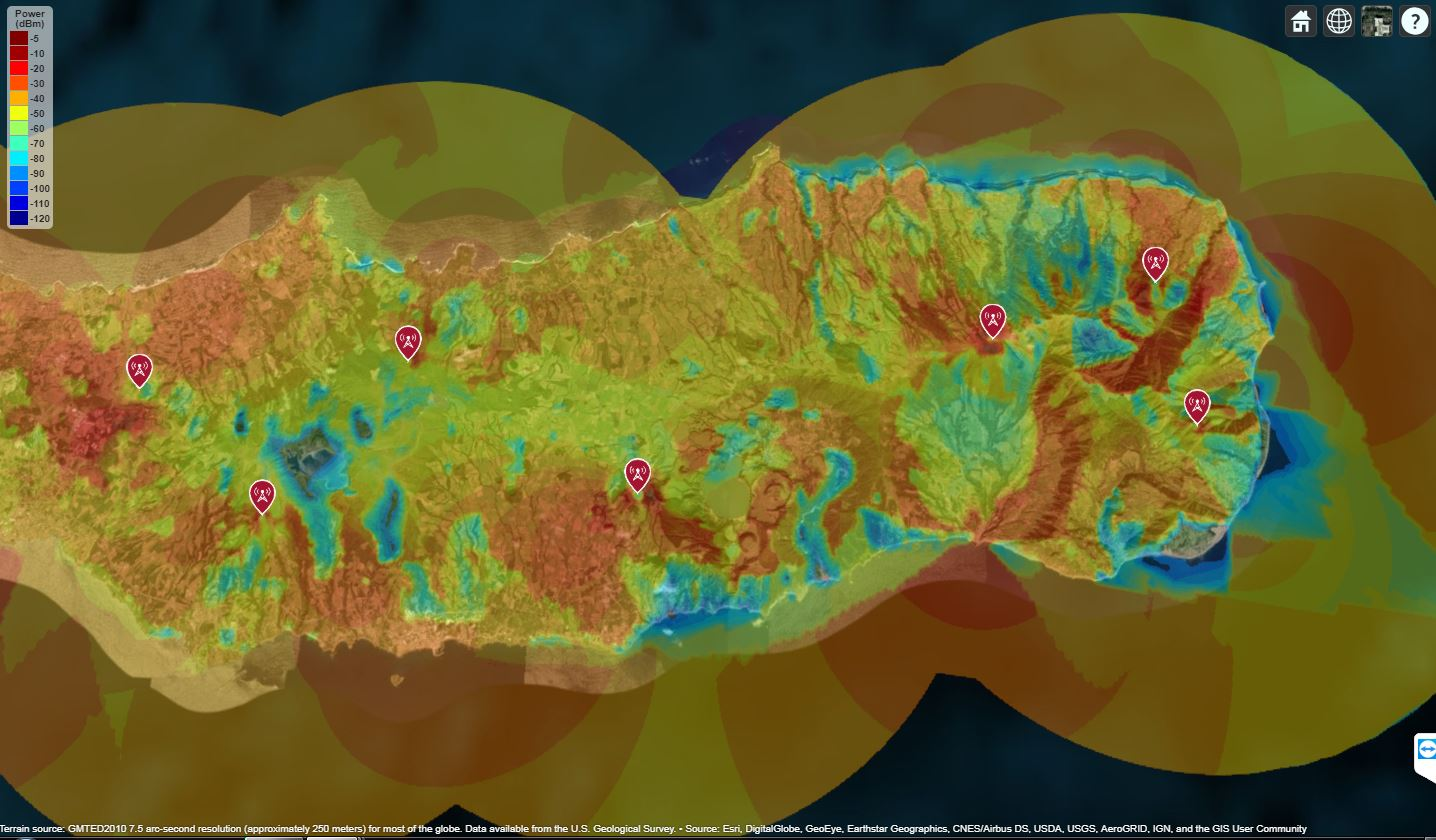
\includegraphics[width=0.45\textwidth]{RecetorEstaticoSemfogoII.JPG}
    \caption{Coverage for a static receiver without fire attenuation - II}
    \label{fig:estaticosemfogoOeste}
\end{figure} 
\FloatBarrier \noindent 
One can see that in this case the coverage reaches almost 100\% of the island area.

\section{Conclusions} \noindent
With these simulations, it is possible to extract valuable information.  In the first scenario, 96.54\% of the island and 99.08\% of the population are covered.  The second case establishes a covered area of 97.82\% and covers 99.15\% of the population.  The third scenario has a covered area of 98.97\% and a covered population of 99.42\%. Finally, the last case has the best coverage values, with 99.44\% of covered area and approximately 100\% of the population is covered. 
\addtolength{\textheight}{-12cm}   % This command serves to balance the column lengths
                                  % on the last page of the document manually. It shortens
                                  % the textheight of the last page by a suitable amount.
                                  % This command does not take effect until the next page
                                  % so it should come on the page before the last. Make
                                  % sure that you do not shorten the textheight too much.

%%%%%%%%%%%%%%%%%%%%%%%%%%%%%%%%%%%%%%%%%%%%%%%%%%%%%%%%%%%%%%%%%%%%%%%%%%%%%%%%



%%%%%%%%%%%%%%%%%%%%%%%%%%%%%%%%%%%%%%%%%%%%%%%%%%%%%%%%%%%%%%%%%%%%%%%%%%%%%%%%



%%%%%%%%%%%%%%%%%%%%%%%%%%%%%%%%%%%%%%%%%%%%%%%%%%%%%%%%%%%%%%%%%%%%%%%%%%%%%%%%
% \section*{APPENDIX}

% Appendixes should appear before the acknowledgment.

% \section*{ACKNOWLEDGMENT}

% The preferred spelling of the word ``acknowledgment'' in America is without an ``e'' after the ``g''. Avoid the stilted expression, ``One of us (R. B. G.) thanks . . .''  Instead, try ``R. B. G. thanks''. Put sponsor acknowledgments in the unnumbered footnote on the first page.



%%%%%%%%%%%%%%%%%%%%%%%%%%%%%%%%%%%%%%%%%%%%%%%%%%%%%%%%%%%%%%%%%%%%%%%%%%%%%%%%

% References are important to the reader; therefore, each citation must be complete and correct. If at all possible, references should be commonly available publications.



\begin{thebibliography}{99}

\bibitem{c1} Luis M. Correia, ``Propagations Models'' 	Slides from Mobile Communication Systems, IST.
\bibitem{c2} W.-K. Chen, Linear Networks and Systems (Book style).	Belmont, CA: Wadsworth, 1993, pp. 123--135.
\bibitem{c3} H. Poor, An Introduction to Signal Detection and Estimation.   New York: Springer-Verlag, 1985, ch. 4.

\end{thebibliography}




\end{document}
